\begin{figure}[t]
\centering
% Round 38 rebuild.  Three reviews (rounds 19, 26, 38) asked for the *inference* diagram as the
% centrepiece rather than a results ladder, the last one drawing it himself.  It already existed twice --
% as a \fbox tabular on page 2 of \S1 and, in results form, here -- so that round CONSOLIDATED the two:
% the left column became the decision chain the page-2 box had carried, and the right columns kept what
% this figure already had, the published result that settles each step.
%
% Round 46 SPLITS THAT BACK APART, and the reason is worth recording because it reverses a predecessor.
% The reviewer asked for two things that turned out to be one object: a "one-picture audit workflow" in
% the first 30 seconds (his #3) and for THIS figure to be simplified until it answers only "what does the
% audit let me conclude?" (his #13).  Measured: the workflow picture existed TWICE -- welded to this
% results ladder on page 3, and again as figure_procedure.tex, which \S3.4 and the conclusion cite and
% which the .aux put on page 16, i.e. BEHIND the references.  A reviewer who read all 94 pages still
% asked for the picture, which makes this a routing/consolidation defect and not a missing figure.  So
% the chain (d0--d4, the two exits, the terminus box, and header 1) moves to figure_audit.tex, which
% \S1 \input{}s and which lands on page 2; what stays here is the ladder alone.
%
% The three level NAMES used to ride inside the chain's d2 box.  They are not dropped: they become this
% figure's left column, which is also what pays for the split -- see the geometry note.
%
% GEOMETRY WARNING, carried from round 15, re-affirmed 38, and the binding constraint on this edit.
% \resizebox scales by WIDTH, so a NARROWER picture renders TALLER and costs body lines.  Natural width
% here is set by the verdict column (\wx=13.20 plus the widest verdict line, rung 3's ~3.44cm), NOT by
% the chain, so deleting the chain must NOT be followed by shifting the ladder left: keeping x fixed and
% filling the vacated 0.15--3.85cm with the level column holds the width at ~16.6cm while the height
% falls from ~5.85cm to ~4.15cm.  That is where the saved lines come from -- the aspect ratio, 2.84 ->
% 4.0.  The bar-label column is right-anchored at \bx, so \bx must clear the widest system-name line
% (~2.5cm from x=4.00) plus the widest label ("operator/arity bag", ~1.95cm); at 8.60 they clear by
% ~0.2cm.  A collision here is invisible to pdftotext and to every gate in this repo -- render the page
% and look at it after any change.
\resizebox{\textwidth}{!}{%
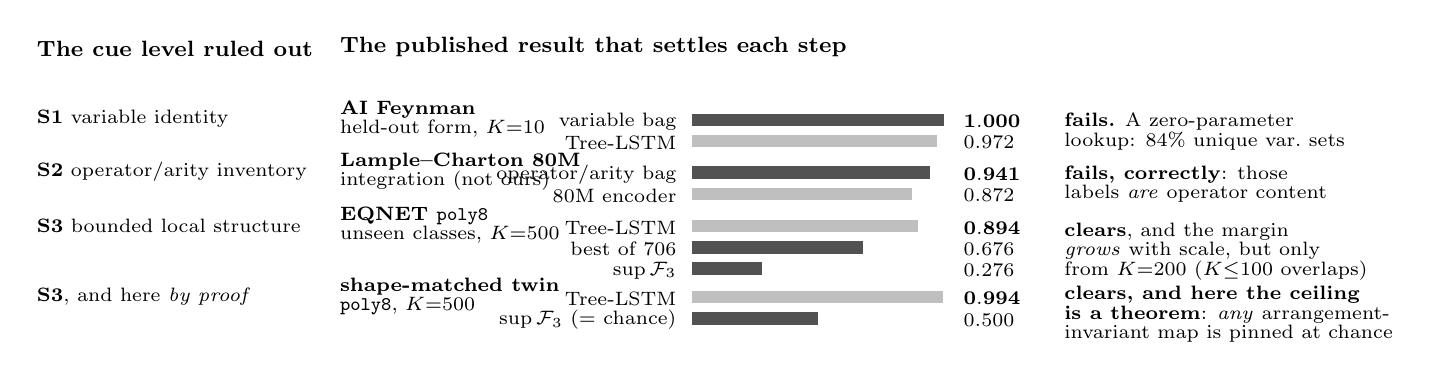
\begin{tikzpicture}[
  font=\footnotesize,
  hdr/.style={font=\footnotesize\bfseries},
  lev/.style={anchor=west, align=left, font=\scriptsize},
  sysname/.style={anchor=west, align=left, font=\scriptsize},
  blab/.style={anchor=east, font=\scriptsize},
  bval/.style={anchor=west, font=\scriptsize},
  verd/.style={anchor=west, align=left, font=\scriptsize},
]
\def\bx{8.60}      % bar origin
\def\bw{3.20}      % bar width at 1.000
\def\vx{11.92}     % value column
\def\wx{13.20}     % verdict column

% Header 1 must fit inside 0.15--3.90cm, i.e. left of the evidence column: at \footnotesize\bfseries
% "The inference a score licenses" measures ~4.35cm and overprinted header 2.  Do not lengthen it.
\node[hdr, anchor=south west] at (0.15, 0.55) {The cue level ruled out};
\node[hdr, anchor=south west] at (4.00, 0.55) {The published result that settles each step};

% ================= S1 =================
\node[lev] at (0.15, -0.12) {\textbf{S1} variable identity};
\node[sysname] at (4.00, -0.12) {\textbf{AI Feynman}\\[-1pt]held-out form, $K{=}10$};
\node[blab] at (\bx-0.08, -0.15) {variable bag};
\fill[black!68] (\bx, -0.21) rectangle ++(1.000*\bw, 0.16);
\node[bval] at (\vx, -0.15) {$\mathbf{1.000}$};
\node[blab] at (\bx-0.08, -0.42) {Tree-LSTM};
\fill[black!25] (\bx, -0.48) rectangle ++(0.972*\bw, 0.16);
\node[bval] at (\vx, -0.42) {$0.972$};
\node[verd] at (\wx, -0.28) {\textbf{fails.} A zero-parameter\\[-1pt]lookup: $84\%$ unique var.\ sets};

% ================= S2 =================
\node[lev] at (0.15, -0.79) {\textbf{S2} operator/arity inventory};
\node[sysname] at (4.00, -0.79) {\textbf{Lample--Charton 80M}\\[-1pt]integration (not ours)};
\node[blab] at (\bx-0.08, -0.82) {operator/arity bag};
\fill[black!68] (\bx, -0.88) rectangle ++(0.941*\bw, 0.16);
\node[bval] at (\vx, -0.82) {$\mathbf{0.941}$};
\node[blab] at (\bx-0.08, -1.09) {80M encoder};
\fill[black!25] (\bx, -1.15) rectangle ++(0.872*\bw, 0.16);
\node[bval] at (\vx, -1.09) {$0.872$};
\node[verd] at (\wx, -0.95) {\textbf{fails, correctly}: those\\[-1pt]labels \emph{are} operator content};

% ================= S3 =================
\node[lev] at (0.15, -1.47) {\textbf{S3} bounded local structure};
\node[sysname] at (4.00, -1.47) {\textbf{EQNET \texttt{poly8}}\\[-1pt]unseen classes, $K{=}500$};
\node[blab] at (\bx-0.08, -1.50) {Tree-LSTM};
\fill[black!25] (\bx, -1.56) rectangle ++(0.894*\bw, 0.16);
\node[bval] at (\vx, -1.50) {$\mathbf{0.894}$};
% Round 47, found on the COLD READ of pages 1--5 as a unit, and it is this figure failing the paper's
% own title.  This rung's tallest DARK bar was the full-token bag at $0.517$, so the picture showed the
% encoder clearing its strongest visible control by $+0.377$ -- while the abstract (page 1), the
% "Strongest admissible control" column of Table~\ref{tab:entitlements} (page 5) and \S\ref{sec:structural_scale}
% all quote the SEARCHED composite, $0.676$, and the margin $+0.22$.  Three of the four rungs agree with
% that table cell for cell; this one did not, and it was the paper's headline cell.
%   Round 39 put the $0.517$ bar here for exactly this reason and wrote the principle down in
% methodology.tex: "Omitting it would have let this paragraph quote $+0.874$ as the margin while a
% stronger admissible control sat at $+0.377$ in Figure~\ref{fig:framework} -- precisely the error the
% paragraph condemns."  Round 41 then raised the top of that chain to the searched composite in the
% abstract, in \S\ref{sec:not_control_task} and in \S\ref{sec:structural_scale}, and left the figure at
% the catalogued line -- and pinned $0.517$ into check_figure_provenance.py, so the gate was enforcing
% the stale top.  Both the number and its pin move together here.
%   Admissible, and a non-member: the composite is order-blind and twin-gated but is not one of
% Definition~\ref{def:audit_complete}'s seven, so it does NOT set $\sup\mathcal{F}_3$, which stays $0.276$
% on the bar below (Appendix~\ref{app:adversarial_family}, "it does not widen Def.~1").  Listing a
% non-member here is this figure's existing practice -- $0.517$ was one too -- and the stronger
% non-member is the honest one to draw.  $0.517$ is not lost: \S\ref{sec:not_control_task} prints the
% whole six-number chain, and Table~\ref{tab:holdout_ceiling} prints it beside the composite.
%   GEOMETRY, and it is why this fix is a relabel rather than a fourth bar.  A fourth bar costs ~0.27cm
% of tikz height, ~6.4pt rendered at this picture's ~0.84 scale, against page 3's 6.624pt of slack --
% a 0.2pt margin, with pages 4 and 5 at 0.000.  A relabel costs nothing: same node count, same y
% coordinates, and the picture's natural width is set by rung 3's verdict line (97.75pt), not here.
% The bar grows to $0.676{\times}3.20 = 2.16$cm, ending at $10.76 < \vx$; the label is 14 characters
% against the 18 of "operator/arity bag", so the right-anchored label column starts at ~6.97cm and
% still clears the sysname column's 6.50cm.  "best composite" is Appendix~\ref{app:adversarial_family}'s
% own noun phrase, which is what the provenance gate now pins it to.
% Round 49, his \S10: elevate the adversarial-search result.  The ladder was already drawn -- three
% ascending bars, on page 3, since round 47 -- but the label gave no sign that the middle bar came from
% a SEARCH, so the strongest thing about it was invisible: a reader read it as one more hand-picked
% baseline.  "best of 706" is the search's own size (r101 `n_distinct_candidates_scored`).
% GEOMETRY: the comment above prices this column at 18 characters MAXIMUM -- "operator/arity bag" is
% 18 and starts the right-anchored column at exactly the sysname column's 6.50cm.  So "best of 706
% searched" (20) and "best of 706 unions" (18, touching) are both unavailable; this is 11, shorter than
% the 14 it replaces, so the constraint is strictly relaxed.  The count 28 (primitives, not composites)
% is carried by \S4.2's opening sentence instead, and both numbers are in Appendix BB.
% The provenance was NOT added to the caption: the caption's last line has under 40pt of tail room, so
% the clause costs a line (~9pt) against page 3's 6.624pt of slack, with pages 4 and 5 at 0.000.
% check_figure_provenance.py does not key on this label -- its BARS tuples assert value-to-appendix-row
% only, and `barlab` is unpacked and never used (checked; the round-47 comment above overstates it).
\node[blab] at (\bx-0.08, -1.77) {best of 706};
\fill[black!68] (\bx, -1.83) rectangle ++(0.676*\bw, 0.16);
\node[bval] at (\vx, -1.77) {$0.676$};
% SOURCE OF TRUTH for this bar: appendix_domain_guards.tex Table~\ref{tab:poly8_unseen}, the row
% "Bag ($\sup\mathcal{F}_3$, the audit statistic)", K=500 column -> 0.276.  Round 39 corrected this from
% 0.277, which is the row BELOW it, "Bag (tree-local, S3; $\notin\mathcal{F}_3$)" -- a descriptor
% Definition~\ref{def:audit_complete} does not enumerate, so it cannot set the ceiling this figure labels.
% Round 38's check decoded each bar's fraction and compared it to the number printed beside it; both read
% 0.277, consistent and wrong.  CHECK EVERY VALUE HERE AGAINST ITS APPENDIX ROW, not against its own bar.
\node[blab] at (\bx-0.08, -2.04) {$\sup\mathcal{F}_3$};
\fill[black!68] (\bx, -2.10) rectangle ++(0.276*\bw, 0.16);
\node[bval] at (\vx, -2.04) {$0.276$};
\node[verd] at (\wx, -1.80) {\textbf{clears}, and the margin\\[-1pt]\emph{grows} with scale, but only\\[-1pt]from $K{=}200$ ($K{\leq}100$ overlaps)};

% ================= the twin: the rung whose ceiling is a THEOREM =================
\node[lev] at (0.15, -2.37) {\textbf{S3}, and here \emph{by proof}};
\node[sysname] at (4.00, -2.37) {\textbf{shape-matched twin}\\[-1pt]\texttt{poly8}, $K{=}500$};
\node[blab] at (\bx-0.08, -2.40) {Tree-LSTM};
\fill[black!25] (\bx, -2.46) rectangle ++(0.994*\bw, 0.16);
\node[bval] at (\vx, -2.40) {$\mathbf{0.994}$};
\node[blab] at (\bx-0.08, -2.67) {$\sup\mathcal{F}_3$ ($=$ chance)};
\fill[black!68] (\bx, -2.73) rectangle ++(0.500*\bw, 0.16);
\node[bval] at (\vx, -2.67) {$0.500$};
% Round 41, R1 \S12 ("you only ruled out the explanations you decided in advance to include"): this cell
% said "every order-blind MEMBER", i.e. family-relative, when Prop.~\ref{prop:twin_exact} proves the
% quantifier is over EVERY arrangement-invariant map, declared or not.  WIDTH-SAFE, and that is not a
% guess: \resizebox scales by width, so the picture's natural width is set by the WIDEST verdict line,
% which is rung 3's "from K=200 (K<=100 overlaps)" at 97.75pt.  The two lines below measure 89.71pt and
% 93.44pt at \scriptsize, so the bounding box, the scale factor and every page below are untouched.
\node[verd] at (\wx, -2.60) {\textbf{clears, and here the ceiling}\\[-1pt]\textbf{is a theorem}: \emph{any} arrangement-\\[-1pt]invariant map is pinned at chance};

\end{tikzpicture}}
% Round 39: the caption's second sentence spelled out the left column in prose, and \S1's new
% fourth paragraph now states the twin's by-proof ceiling and tree-edit distance verbatim.  Both
% were cut here rather than in \S1: the figure renders the left column itself, and page 2 is where
% the reviewer asked for the twin.  $0.723$ STAYS -- check_figure_provenance.py asserts it here.
%
% Round 40, R2 ("move the twin to the absolute centre"): the twin's by-proof ceiling was the caption's
% SECOND sentence, behind the bar-shading legend, so the entry-point figure opened on a rendering note.
%
% Round 46, his #4 ("every section should start with its finding") applied to a caption: the finding
% now opens it, and the ladder's job -- one real benchmark per step of the audit; two of the four rungs
% are other people's published results and two are ours on EQNET's data -- is stated second,
% pointing at Figure~\ref{fig:audit} rather than re-drawing it.  The class-unit clause is his #17.
\caption{\textbf{The twin is the one rung whose ceiling is known by proof}: \emph{any}
arrangement-invariant representation is pinned at chance, and tree-edit distance, the strongest
order-sensitive \emph{non}-member, reaches only $0.723$. Each rung settles one step of
Figure~\ref{fig:audit}'s chain, at the level named on the left; dark bars are non-learned controls,
light bars trained models, and the unit of inference is the equivalence class on \texttt{poly8} and the
individual expression above it. \textbf{Coverage is not a rung} but one of the five novelty axes costed
in \S\ref{sec:loso}, and not a monotone gate; its ordering fails on \texttt{boolean8}.}
\label{fig:framework}
\end{figure}
